\documentclass[conference]{IEEEtran}
\IEEEoverridecommandlockouts
\usepackage{graphicx}
\usepackage{textcomp}
% The preceding line is only needed to identify funding in the first footnote. If that is unneeded, please comment it out.
\usepackage{cite}
\usepackage{amsmath,amssymb,amsfonts}
\usepackage{algorithmic}
\usepackage{graphicx}
\usepackage{textcomp}
\usepackage{xcolor}
\def\BibTeX{{\rm B\kern-.05em{\sc i\kern-.025em b}\kern-.08em
    T\kern-.1667em\lower.7ex\hbox{E}\kern-.125emX}}
\begin{document}



\title{Artificial intelligence for anomaly detection in IoMTs\\
}

\author{\IEEEauthorblockN{Mickael Mohammed}
\IEEEauthorblockA{\textit{Student in Cybersecurity and e-Health’s Master Degree} \\
\textit{Université Paris Cité}\\
Paris, France \\
mickael.mohammed@etu.u-paris.fr}
\and
\IEEEauthorblockN{Osman Salem}
\IEEEauthorblockA{\textit{Teacher Researcher at the Borelli Center} \\
\textit{Université Paris Cité}\\
Paris, France \\
osman.salem@u-paris.fr}


}






\author{%
    \begin{tabular}{@{}c@{}}
    \IEEEauthorblockN{Mickael Mohammed} \\
    \begin{tabular}{@{}c@{}}
    \textit{Student in Cybersecurity} \\
    \textit{and e-Health’s Master Degree}\\
    \end{tabular} \\
    \textit{Université Paris Cité}\\
    Paris, France \\
    mickael.mohammed@etu.u-paris.fr
    \end{tabular}
    \begin{tabular}{@{}c@{}}
    \IEEEauthorblockN{Osman Salem} \\
    \begin{tabular}{@{}c@{}}
    \textit{ Researcher at the Borelli Center} \\
 
    \end{tabular} \\
    \textit{Université Paris Cité}\\
    Paris, France \\
    osman.salem@u-paris.fr
    \end{tabular}
    \begin{tabular}{@{}c@{}}
    \IEEEauthorblockN{Ahmed Mehaoua} \\
    \begin{tabular}{@{}c@{}}
    \textit{ Researcher at the Borelli Center} \\
    \end{tabular} \\
    \textit{Université Paris Cité}\\
    Paris, France \\
    ahmed.mehaoua@u-paris.fr
    \end{tabular}
}


\maketitle

\begin{abstract}
The exponential development and widespread emergence of the Internet of Medical Things (IoMT) have led to a growing need for effective anomaly detection techniques to ensure the reliability and security of healthcare systems. This article provides a review of existing machine learning and deep learning algorithms for anomaly detection in IoMT, followed by the presentation of a novel approach combining ARIMA for predicting health parameter values and a decision tree for anomaly detection. This hybrid approach aims to improve the accuracy and efficiency of anomaly detection in IoMT by leveraging both time series models and the discriminative features of decision trees. The preliminary results of this approach are presented and discussed, highlighting its potential to enhance early detection of anomalies in IoMT and contribute to safer and more reliable healthcare.
\end{abstract}

\begin{IEEEkeywords}
Internet of Medical Things, machine learning, deep learning, ARIMA, decision tree, anomaly detection
\end{IEEEkeywords}

\section{Introduction}
Anomaly detection on IoT devices in the healthcare domain has seen significant advancements with the use of AI (Artificial Intelligence). IoT devices in healthcare, known as IoMT (Internet of Medical Things), generate real-time data through wearables, implants, and home health monitors. This data provides an opportunity for continuous patient monitoring and the detection of anomalies indicating critical health conditions or deteriorations.

AI techniques, such as machine learning and deep learning, have been widely utilized for anomaly detection in IoMT data. These approaches model normal behavior patterns and identify atypical behaviors suggesting health issues. Anomaly detection methods employ tailored algorithms to handle various types of data from IoMT devices, including time series, unstructured, or multidimensional data. Common approaches include statistics-based methods, supervised learning methods like Support Vector Machines (SVM), and unsupervised learning methods like recurrent neural networks (RNN).

However, there are several challenges in anomaly detection on IoMT devices, such as managing real-time data, accounting for individual variations, detecting contextual anomalies, and reducing false positives. Ongoing research aims to develop more sophisticated AI models and advanced preprocessing techniques to improve anomaly detection accuracy and provide early alerts in critical situations.

The goal of anomaly detection is to observe abnormal data generated by medical sensors during a specific time frame. These exceptional data can arise from either a transient or permanent malfunction of the medical sensor or may be attributed to a cyber attack.

In a scenario where a patient is unwell but does not require immediate medical attention, multiple medical sensors, acting as interconnected devices, continuously monitor the patient's health status in real time. Detecting anomalies in health data helps prevent unnecessary alarms from being raised at hospitals or emergency rooms, allowing the focus to remain on patients in critical condition.

These interconnected medical devices function autonomously and communicate with each other through a shared network, known as the Internet of Medical Things (IoMT). The computer receives multiple series of vital health parameter values periodically. After analyzing the medical data, the computer assesses the patient's health condition and identifies any false health data emitted by a sensor. The computer's role includes detecting anomalies in the data while issuing an alarm in the event of a genuine critical condition.

If a sensor sporadically emits abnormal data with a negligible error rate, the computer continues to receive values from that sensor. However, if the sensor persistently emits abnormal and erroneous data, the computer excludes that sensor's data when assessing the patient's health status. The computer then notifies the relevant medical committee about the malfunctioning state of the sensor.

In this article, we will first review the state of the art of existing anomaly detection techniques, including machine learning algorithms for prediction such as SVM and KNN, and deep learning algorithms such as RNN and CNN. We will then present our own approach, which consists of using Arima on time series of health parameter values to predict subsequent values and determine the patient's health status at a given period. The use of Arima will be followed by the application of a decision tree on the values predicted by Arima to possibly detect data anomalies emitted by a medical sensor.

Finally, we will compare the accuracy of our approach combining the application of Arima and a decision tree on a medical health dataset with the accuracy of existing machine learning and deep learning algorithms such as SVM and RNN applied on the same medical health dataset.

\section{Related Work}



The Internet of Medical Things (IoMT) is proving to be a revolution in the healthcare sector, enabling real-time collection of data from medical sensors, monitoring devices, and patients. However, this abundance of data poses a major challenge: how to effectively detect anomalies that may indicate critical medical conditions or IoMT device malfunctions?


\subsection{Automatic machine learning approaches for anomaly detection:}
Traditional machine learning approaches for anomaly detection in IoMT have proven to be effective in many cases. Among these, clustering methods such as k-means and DBSCAN have been used to group data and identify unusual observations \cite{b1}. Support Vector Machines (SVM) and k-Nearest Neighbors (KNN) are two additional commonly used techniques for anomaly detection in IoMT.
ese approaches offer acceptable performance, but their effectiveness can be limited due to the complexity and dynamic nature of IoMT data\cite{b2}.
\begin{itemize}

\item Among machine learning algorithms, k-nearest neighbors (KNN) is a simple and widely used approach. KNN assigns a label to a new example based on the labels of its k nearest neighbors in the feature space. It is effective in detecting anomalies in IoMT when anomalies clearly stand out from normal data.
\item 
Support vector machines (SVMs) are another commonly used automatic machine learning method for anomaly detection. The SVM algorithm finds the optimal hyperplane that separates normal data from anomalies in a higher-dimensional space. It is effective when anomalies are linearly separable from normal data\cite{b3}.

\end{itemize}


\subsection{Deep learning approaches for anomaly detection:}
With the emergence of deep learning, new approaches have been developed to enhance anomaly detection in IoMT. Convolutional neural networks (CNNs) have been successfully applied to analyze medical images, enabling accurate detection of lesions, tumors, and other anatomical anomalies\cite{b4} \cite{b5}. Recurrent neural networks (RNNs) have been used to model temporal sequences in IoMT data, allowing for anomaly detection in biomedical signals and clinical time series data\cite{b6}. Generative adversarial networks (GANs) have also been explored to generate synthetic reference data for improved anomaly detection in IoMT\cite{b7}. These deep learning approaches have demonstrated promising performance, but often require massive datasets and significant computational resources\cite{b8}.
\begin{itemize}
\item 
Convolutional neural networks (CNNs) are widely used for medical image analysis in IoMT. They are capable of learning complex visual features from images and detecting anomalies such as lesions or tumors. CNNs use convolution and pooling layers to progressively extract features at different scales and classify them using fully connected layers.
\item 

Recurrent neural networks (RNNs) are used to model temporal sequences in IoMT data. They are effective in detecting anomalies in biomedical signals and clinical time series data\cite{b9}. RNNs have recurrent connections that allow them to retain short and long-term information, which is useful for detecting abnormal patterns in sequences.

\end{itemize}

\vspace{6pt}
Each algorithm has specific advantages and limitations. KNN is simple to understand and implement, but it can be sensitive to data density. SVMs are effective at separating classes but may be less suitable when data is highly nonlinear. CNNs are capable of learning complex visual features but require massive datasets and significant computational resources. RNNs are well-suited for modeling sequences but may be sensitive to long-term dependencies.

\section{Proposed Approach}
Our approach entails initially applying ARIMA to a time series of a single health parameter's values in order to forecast subsequent values. 

\subsection{Introduction to Arima Prediction Algorithm}

ARIMA (AutoRegressive Integrated Moving Average) is a widely used time series forecasting algorithm known for its effectiveness in capturing and predicting trends and patterns in data. It combines autoregressive (AR), differencing (I), and moving average (MA) components to model and forecast time series data. ARIMA has three main parameters: $p$, $d$, and $q$. 
\begin{itemize}
\item 
The parameter $p$ represents the order of the autoregressive component
\item $d$ represents the degree of differencing
\item $q$ represents the order of the moving average component. 
\end{itemize}
By selecting appropriate values for these parameters, ARIMA can capture both short-term and long-term dependencies in the data.

One notable feature of ARIMA is its ability to handle non-stationary data by differencing, making it suitable for time series data with trends or seasonality.

This distinguishes ARIMA from other prediction algorithms like linear regression, which assumes a linear relationship between variables. ARIMA's power lies in its ability to capture complex temporal patterns and make accurate predictions, even when the data exhibits non-linear trends or irregularities.
ARIMA finds utility in predicting various health parameters such as SP (Systolic Blood Pressure), O2 (Oxygen Saturation), HR (Heart Rate), and BP (Blood Pressure). These parameters are often measured at regular intervals, making them suitable for time series analysis. 

ARIMA can analyze the historical data of these health parameters and provide forecasts for future values. This capability is particularly valuable in healthcare applications where predicting vital signs and health metrics in advance can assist in early detection of anomalies, monitoring patient conditions, and informing medical interventions. 

ARIMA's versatility and adaptability make it a valuable tool for healthcare professionals and researchers in predicting health parameter values and aiding in decision-making processes.
ARIMA can be used for anomaly detection in a medical health game.
\subsection{Procedure for applying ARIMA on the medical dataset and calculating ARIMA's accuracy}

One common application of ARIMA for anomaly detection is to compare the model's predictions with the actual values. If an observed value deviates significantly from ARIMA's prediction, it can be considered an anomaly.



By using ARIMA, we can model and forecast the expected values of health parameters, such as systolic blood pressure, oxygen saturation, or heart rate, based on historical data. 
ARIMA operates based on the concept of a window size, meaning it takes as input a sublist of values from the entire list of values for a single health parameter. It can then predict the values of the next sublist for that same health parameter, along with a confidence interval within which the upcoming values should fall.
If a real value falls outside the confidence interval predicted by ARIMA, it may indicate an anomaly or unusual behavior.

In this research study, we applied the ARIMA (AutoRegressive Integrated Moving Average) method to a medical health dataset containing time series data of SP02, HR, BP02, and a class indicating the critical or non-critical health state of the patient.
These medical values are derived from a dataset extracted from physioBANK ATM. 

Our goal was to predict the values of health parameters and classify the patient's health state.
For each health parameter, we extracted the respective data and subdivided it into multiple sublists of size 12.

Starting from the first sublist, we utilized ARIMA to predict the next 12 values for the subsequent sublist. By calculating the average of the predicted values, we were able to establish a confidence interval within which the next actual values of the sublist should lie. The next real values outside of this confidence interval may then be considered abnormal.

   \[
   Confidence Interval = [Average - 10\% ; Average + 10\%]
   \] 


This process was iterated for each subsequent sublist, employing the actual values of the following list to predict the subsequent values. Thus, with each iteration, a new confidence interval was obtained for future predictions.

Subsequently, we conducted a comparison between the predicted values of the first sublist and the actual values of the second list. To evaluate the accuracy of ARIMA, we computed the absolute difference between each corresponding actual and predicted value and accumulated these differences into a variable referred to as the "total residual sum".

The precision of ARIMA was then determined using the formula:


\[
Accuracy = 100-\cfrac{\sum{residuals}}{n}
\]




It should be noted that this approach allowed us to assess the precision of ARIMA across the entire dataset. 
Moreover, by utilizing confidence intervals, we were able to estimate the likely range of future actual values for each health parameter, facilitating the detection of potential anomalies.


\begin{figure}
    \centering
    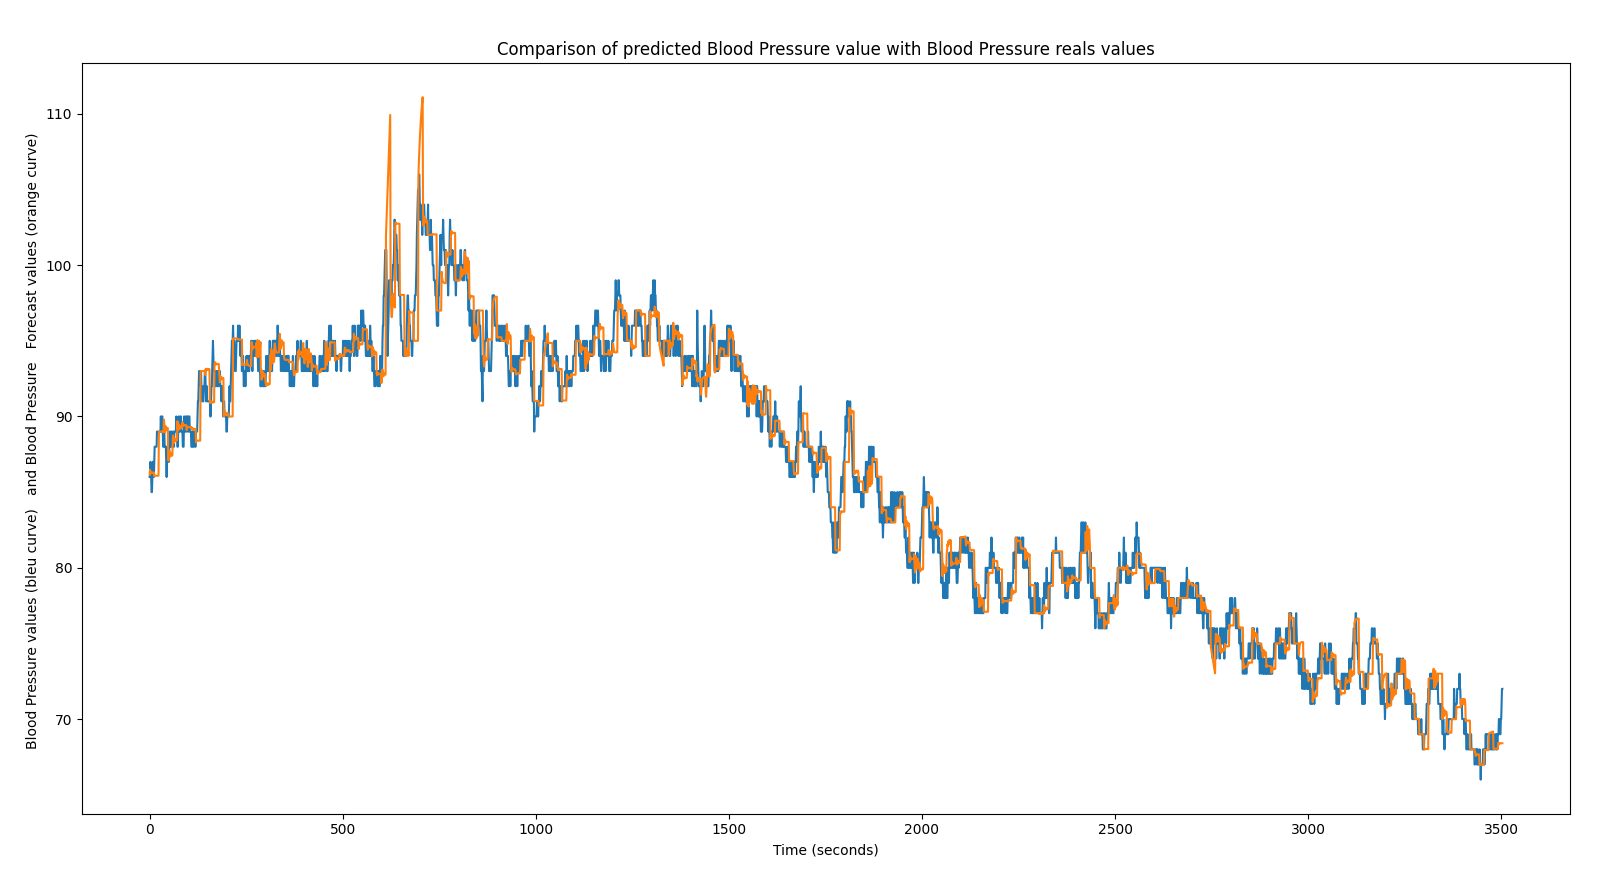
\includegraphics[scale=0.22]{figure1.PNG}
    \caption{Comparison of predicted Blood Pressure values with Blood Pressure reals values as a function of time}
    \label{fig:my_label}
\end{figure}

\begin{figure}
    \centering
    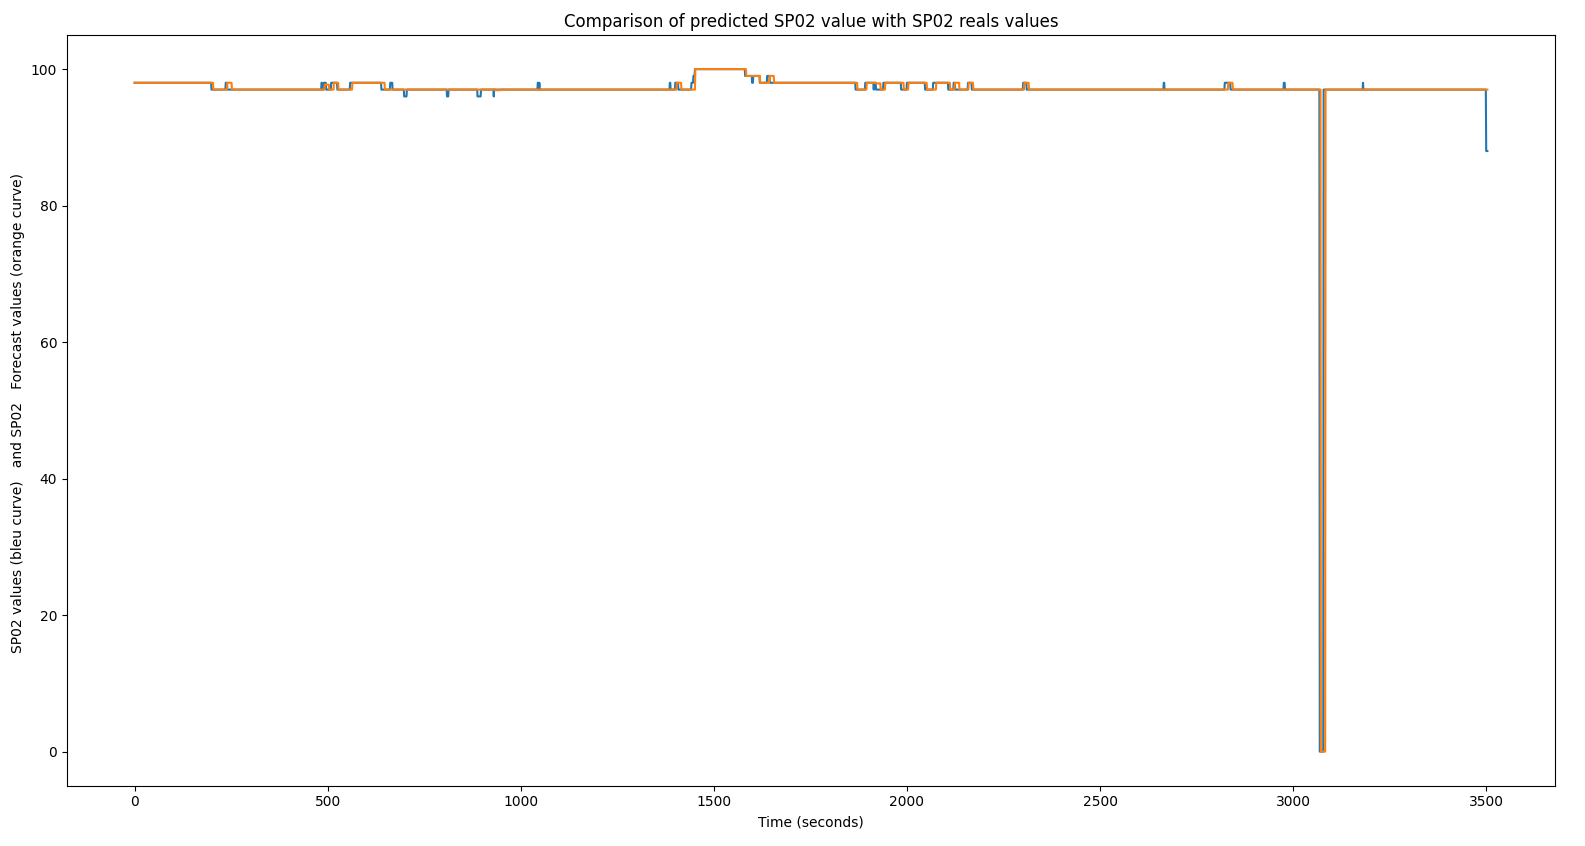
\includegraphics[scale=0.22]{Figure2.PNG}
    \caption{Comparison of predicted SP02 values with SP02 reals values as a function of time}
    \label{fig:my_label}
\end{figure}

\begin{figure}
    \centering
    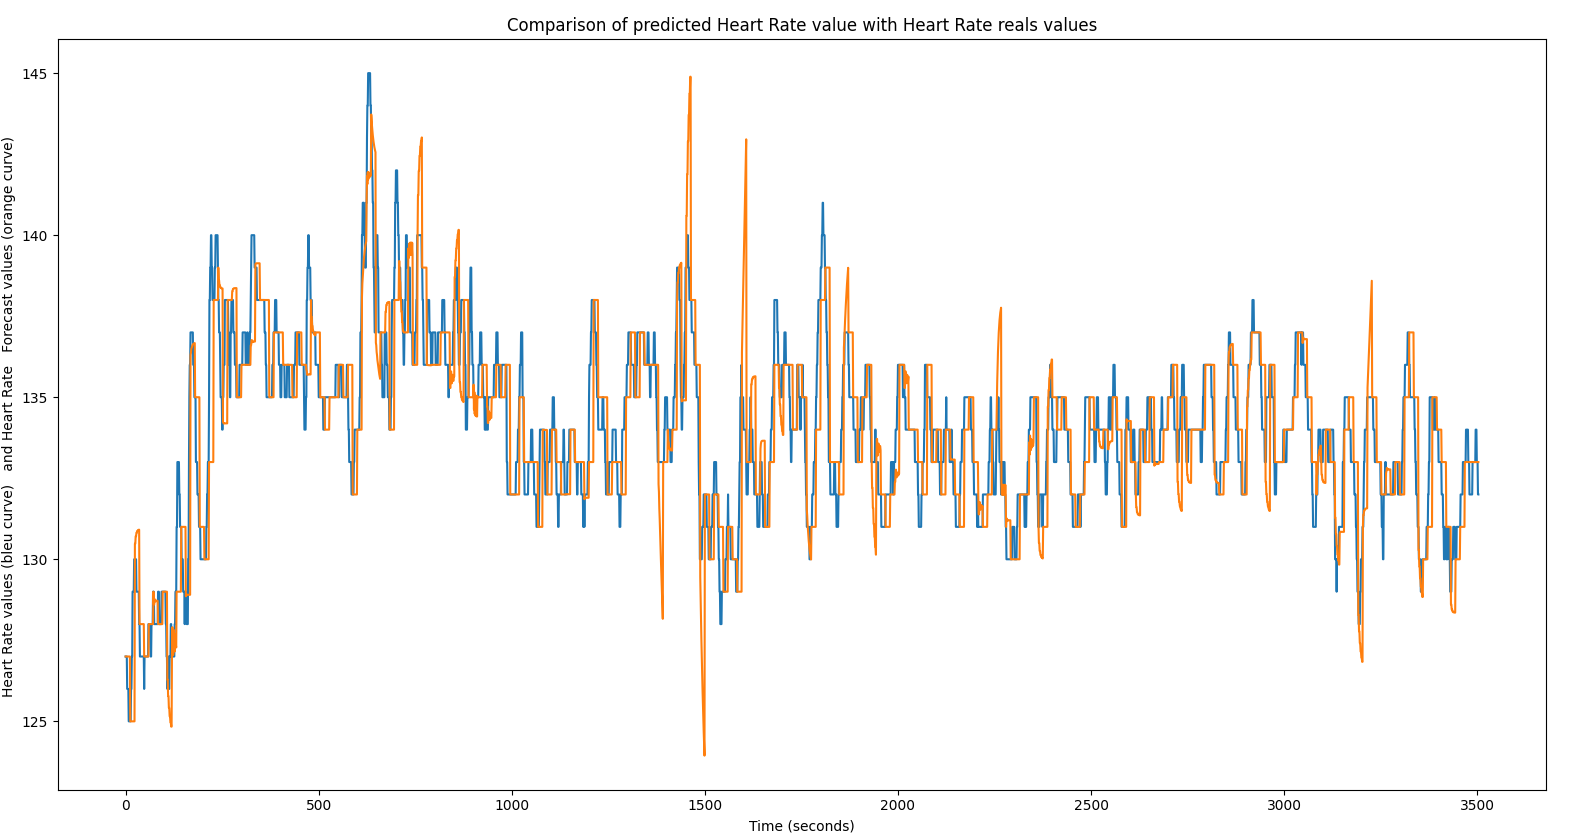
\includegraphics[scale=0.22]{Figure3.PNG}
    \caption{Comparison of predicted Heart Rate values with Heart Rate reals values as a function of time}
    \label{fig:my_label}
\end{figure}


The precision of ARIMA can also be calculated using a different formula. If the predicted value belongs to the same class as the actual measured value, we can consider it a True Positive. For instance, if the actual oxygen level at a given time is measured to be 98\% and ARIMA predicts it as 96\%, we have a True Positive because the predicted value falls within the same class as the actual measured value.
Conversely, if the predicted value belongs to a different class than the actual value, we have a False Positive.
Therefore, another formula to calculate the precision of ARIMA with data of different nature would be:


\[
Accuracy = \cfrac{{True \, positives}}{True \quad positives \quad + \quad Falses \quad positives}
\]
\vspace{3pt}
We found that the accuracy of the Arima model applied to the medical health dataset is 94\%.

In conclusion, the application of ARIMA to the time series data of SP02, HR, and BP02, combined with the prediction of the critical or non-critical health state, yielded promising results. However, it is essential to acknowledge the limitations of ARIMA, including its sensitivity to abrupt variations and unforeseen events. 

However, Arima is only a component of our approach, and this initial accuracy measure of Arima does not fully reflect the effectiveness of our overall approach. To assess the accuracy of our approach comprehensively, we will evaluate the accuracy of the decision tree utilized for class prediction based on the health parameter values predicted by Arima.



\subsection{Decision tree used to predict the class and  to detect health parameters with data anomalies}


Once we have obtained the average of the three sublists of predicted health parameter values, SP02, BP, and HR, we can then determine the class indicating whether the patient's health status is normal or critical based on the values of these health parameters in relation to existing vital thresholds. A blood oxygen saturation below 95\% is critical, a heart rate outside the range of 60 to 120 beats per minute can be serious, and a blood pressure outside the reference range of 90 mmHg to 140 mmHg can also be extremely serious.

Given the correlation between the values of the health parameters, we are also able to detect data anomalies. For instance, it is impossible for a patient to have critically low oxygen saturation and blood pressure with a normal heart rate. Similarly, it is implausible to have a critically high heart rate and blood pressure with normal oxygen saturation.

\begin{figure}[htbp]
    \centering
    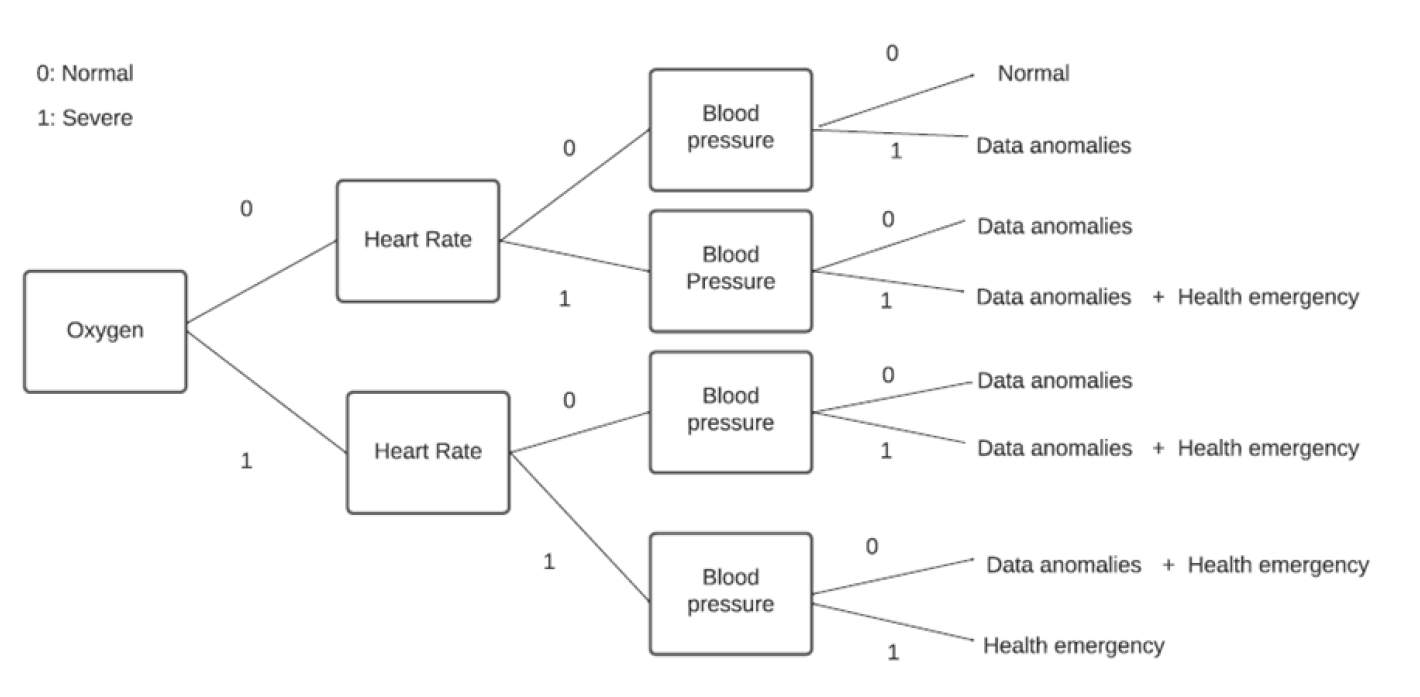
\includegraphics[scale=0.25]{Capture4.PNG}
    \caption{Decision tree}
    \label{fig:my_label}
\end{figure}

We make the assumption that only one sensor, at most, can emit abnormal data. By utilizing a decision tree where the class of each health parameter is known, we can identify which specific health parameter possesses abnormal and false values. In this decision tree, each path represents a distinct rule. For instance, the path 1 0 1 signifies a data anomaly, as it is not possible to have a normal heart rate while simultaneously having critical oxygen levels and a critical blood pressure.

From the decision tree, we will predict the class for each row in the dataset.

To determine the accuracy of the decision tree in predicting the class based on the data predicted by Arima, we will divide the True Positives variable, which represents the total number of correctly predicted classes by our model, by the total number of actual classes.

This calculation will provide us with a measure of how well the decision tree is able to accurately classify the data, considering the predicted values obtained from Arima. By evaluating the ratio of True Positives to the total number of actual classes, we can assess the precision of our approach and gain insights into the effectiveness of the decision tree in class prediction.

 We will be able to evaluate the final accuracy of our model using the decision tree to predict the class based on the predicted values obtained through Arima. We have observed that the accuracy of our model was 93\%.

Please note that the perceived accuracy is considered quite substantial, attesting to the efficacy of our approach.. It indicates that the model is able to correctly predict the class for a large majority of the data instances. This high accuracy suggests that the decision tree model, combined with the predicted values from Arima, is performing well in classifying the data.



\section{Experimental results}
In this paper, we propose an alternative approach for anomaly detection in the IoMT (Internet of Medical Things) domain. In this section, we will evaluate the efficiency of our algorithm using a medical health dataset. To facilitate comparison, we will apply two other algorithms on the same dataset in parallel: one based on Deep Learning (RNN) and the other on Machine Learning (SVM).

For the Artificial Intelligence algorithms, we have divided the dataset into an 80\% training set and a 20\% testing set, while ensuring that the frequency of each class in the original dataset is preserved. This decision is not arbitrary and is based on \cite{b10} to minimize the risk of overfitting.
All our algorithms will be implemented within a Python environment, such as Google Colab or PyCharm's IDE.

\begin{figure}[htbp]
    \centering
    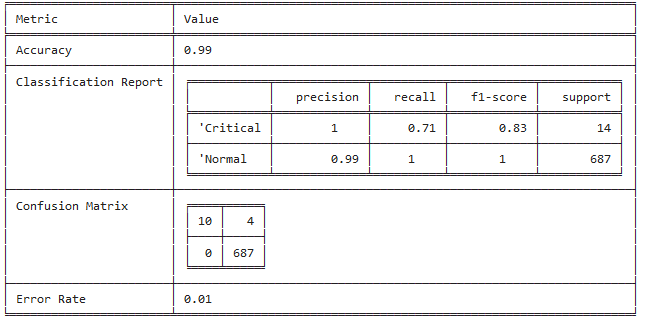
\includegraphics[scale=0.55]{Capture10.PNG}
    \caption{SVM performances}
    \label{fig:my_label}
\end{figure}

\begin{figure}[htbp]
    \centering
    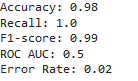
\includegraphics[scale=0.95]{Capture12.PNG}
    \caption{RNN performances}
    \label{fig:my_label}
\end{figure}




We will see that the results of running SVM and RNN on the medical health dataset indicate that SVM has an accuracy of 99\%, while RNN has an accuracy of 98\%.
The accuracy of RNN and SVM is thus superior to that of our model, which has an accuracy of 93\% and combines ARIMA with a decision tree.
The performance of a classification model can also be evaluated by measuring the Area Under the ROC Curve (AUC-ROC), which represents the model's ability to discriminate between positive and negative classes. A model with an AUC-ROC close to 1 is considered to be performing well, indicating a good separation between the classes. On the other hand, an AUC-ROC close to 0.5 suggests random performance of the model, indicating that it is no better than random guessing in distinguishing between the classes.

\begin{figure}[htbp]
    \centering
    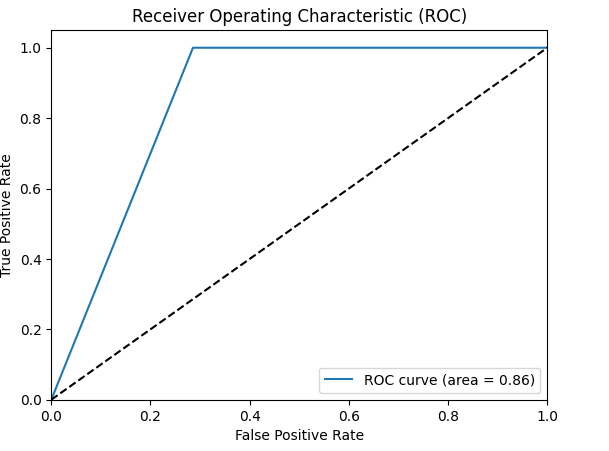
\includegraphics[scale=0.55]{Capture6.PNG}
    \caption{SVM - ROC curve}
    \label{fig:my_label}
\end{figure}
\begin{figure}[htbp]
    \centering
    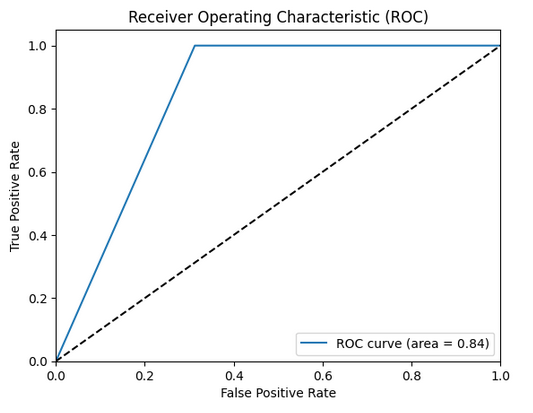
\includegraphics[scale=0.55]{Arima-SVM.PNG}
    \caption{Arima and SVM - ROC curve}
    \label{fig:my_label}
\end{figure}
\begin{figure}[htbp]
    \centering
    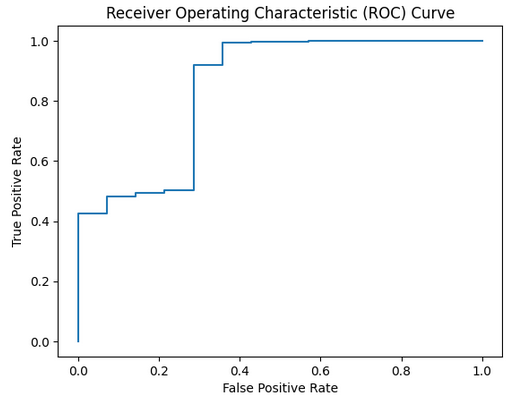
\includegraphics[scale=0.65]{Capture11.PNG}
    \caption{RNN - ROC curve}
    \label{fig:my_label}
\end{figure}
\begin{figure}[htbp]
    \centering
    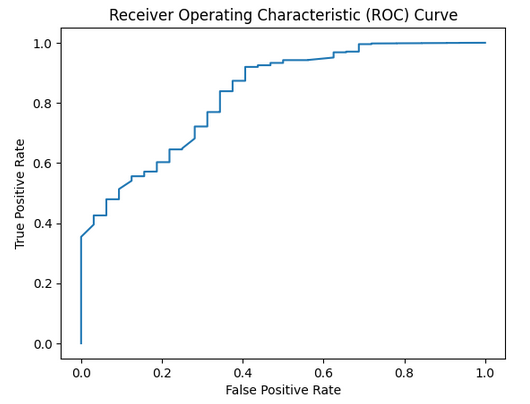
\includegraphics[scale=0.65]{Arima-RNN.PNG}
    \caption{Arima and RNN - ROC curve}
    \label{fig:my_label}
\end{figure}
\begin{figure}[htbp]
    \centering
    \includegraphics[scale=0.65]{Decision Tree-ROC Curve.PNG}
    \caption{Decision Tree - ROC curve}
    \label{fig:my_label}
\end{figure}
\begin{figure}[htbp]
    \centering
    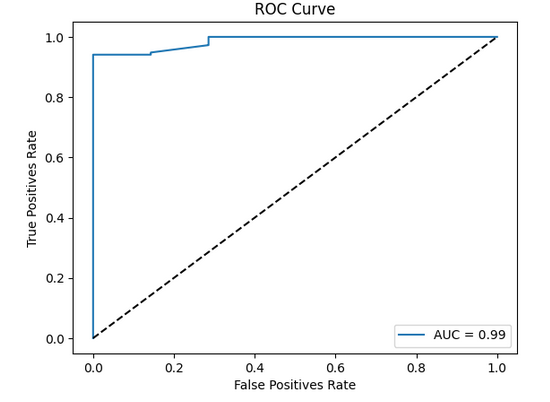
\includegraphics[scale=0.65]{Arima_DecisionTree.PNG}
    \caption{Arima and Decision Tree - ROC curve}
    \label{fig:my_label}
\end{figure}

According to the ROC curves of the prediction algorithms SVM and RNN applied to real healthcare data, it can be observed that the performance of these algorithms seems to be more limited than what is indicated by other performance measures such as accuracy.

\begin{figure}[htbp]
    \centering
    \includegraphics[scale=0.22]{Accuracy.PNG}
    \caption{Comparison of the accuracy of our model with existing prediction algorithms}
    \label{fig:my_label}
\end{figure}

\section{Conclusion}
To conclude in this paper we proposed a new approach for anomaly detection in IOMT using AI.

We observed that our new approach for detecting anomalies in IOMTs, combining the use of Arima and a decision tree with a patient's medical health dataset, was fairly effective, as the accuracy of this model was 94\%.
However, the accuracy of other models using artificial intelligence such as machine learning algorithms like SVM and deep learning algorithms like RNN was higher than our model.

Therefore, we observe that AI can enhance the accuracy of anomaly detection in medical data by utilizing sophisticated algorithms to analyze real-time medical data and identify abnormal patterns or behaviors, ensuring continuous patient monitoring.



\begin{thebibliography}{00}
\bibitem{b1}Ester, M., Kriegel, H.P., Sander, J., & Xu, X. (1996). A density-based algorithm for discovering clusters in large spatial databases with noise. In Proceedings of the Second International Conference on Knowledge Discovery and Data Mining (KDD'96) (pp. 226-231).
\bibitem{b2}Zheng, Y., Liu, J., Wang, W., & Zomaya, A.Y. (2019). A comprehensive survey on the detection methods of anomaly-based Intrusions in the Internet of Things (IoT) paradigm. 
\bibitem{b3}Cortes, C., & Vapnik, V. (1995). Support-vector networks. Machine learning, 20(3), 273-297.
\bibitem{b4}Litjens, G., Kooi, T., Bejnordi, B.E., Setio, A.A.A., Ciompi, F., Ghafoorian, M., van der Laak, J.A., van Ginneken, B., & Sánchez, C.I. (2017). A survey on deep learning in medical image analysis. Medical Image Analysis, 42, 60-88.
\bibitem{b5}Shen, D., Wu, G., & Suk, H.I. (2017). Deep learning in medical image analysis. Annual Review of Biomedical Engineering, 19, 221-248.
\bibitem{b6}Lipton, Z.C., Berkowitz, J., & Elkan, C. (2015). A critical review of recurrent neural networks for sequence learning. arXiv preprint arXiv:1506.00019.
Malhotra, P., Vig, L., Shroff, G., & Agarwal, P. (2015). Long short term memory networks for anomaly detection in time series. In Proceedings of the European Symposium on Artificial 

\bibitem{b7}Schlegl, T., Seeböck, P., Waldstein, S.M., Schmidt-Erfurth, U., & Langs, G. (2017). Unsupervised anomaly detection with generative adversarial networks to guide marker discovery. In International Conference on Information Processing in Medical Imaging (pp. 146-157). Springer, Cham.

\bibitem{b8} Li, X., Chen, T., Wei, W., & Li, J. (2020). Deep learning for anomaly detection: A review. Neurocomputing, 396, 126-141.

\bibitem{b9}Malhotra, P., Vig, L., Shroff, G., & Agarwal, P. (2015). Long short term memory networks for anomaly detection in time series. In Proceedings of the European Symposium on Artificial 

\bibitem{b10}G´eron, A. Hands-On Machine Learning with Scikit-Learn and Tensor Flow: Concepts, Tools, and Techniques to Build Intelligent Systems; O’Reilly Media: Sebastopol, CA, USA, 2017.

\end{thebibliography}
\vspace{12pt}
\color{red}


\end{document}
